%%%%%%%%%%%%%%%%%%%%%%%%%%%%%%%%%%%%%%%%%%%%%%%%%%%%%%%%%%%%%%%%%%%%%%%%%%%%%%%%%%
\begin{frame}[fragile]\frametitle{}
\begin{center}
{\Large Using Open-Source Large Language Models}
\end{center}
\end{frame}

%%%%%%%%%%%%%%%%%%%%%%%%%%%%%%%%%%%%%%%%%%%%%%%%%%%%%%%%%%%%%%%%%%%%%%%%%%%%%%%%%%
\begin{frame}[fragile]\frametitle{}
\begin{center}
{\Large Via LM Studio}
\end{center}
\end{frame}


%%%%%%%%%%%%%%%%%%%%%%%%%%%%%%%%%%%%%%%%%%%%%%%%%%%%%%%%%%%%%%%%%%%%%%%%%%%%%%%%%%
\begin{frame}[fragile]\frametitle{AutoGen: Overview and Configuration}
\begin{itemize}
\item AutoGen leverages OpenAI APIs by default
\item Requires well-structured configuration setup
\item Uses OpenAI and Azure OpenAI models (gpt-4, gpt-3.5-turbo)
\item Configuration includes model, API key, base URL, and version
\item Supports both OpenAI and Azure API types
\end{itemize}
\end{frame}

%%%%%%%%%%%%%%%%%%%%%%%%%%%%%%%%%%%%%%%%%%%%%%%%%%%%%%%%%%%%%%%%%%%%%%%%%%%%%%%%%%
\begin{frame}[fragile]\frametitle{Default Config}

\begin{lstlisting}
openai_config_list = [
    {
        "model": "gpt-4",
        "api_key": "<your OpenAI API key here>"
    },
    {
        "model": "gpt-4",
        "api_key": "<your Azure OpenAI API key here>",
        "api_base": "<your Azure OpenAI API base here>",
        "api_type": "azure",
        "api_version": "2023-07-01-preview"
    },
    {
        "model": "gpt-3.5-turbo",
        "api_key": "<your Azure OpenAI API key here>",
        "api_base": "<your Azure OpenAI API base here>",
        "api_type": "azure",
        "api_version": "2023-07-01-preview"
    }
]
\end{lstlisting}
\end{frame}


%%%%%%%%%%%%%%%%%%%%%%%%%%%%%%%%%%%%%%%%%%%%%%%%%%%%%%%%%%%%%%%%%%%%%%%%%%%%%%%%%%
\begin{frame}[fragile]\frametitle{AutoGen: Basic Usage}
Once you’ve set up the configuration, you can query like this:

\begin{lstlisting}
import autogen
question = "Who are you? Tell it in 2 lines only."
response = autogen.oai.Completion.create(config_list=openai_config_list, prompt=question, temperature=0)
ans = autogen.oai.Completion.extract_text(response)[0]
print("Answer is:", ans)
\end{lstlisting}
\end{frame}

%%%%%%%%%%%%%%%%%%%%%%%%%%%%%%%%%%%%%%%%%%%%%%%%%%%%%%%%%%%%%%%%%%%%%%%%%%%%%%%%%%
\begin{frame}[fragile]\frametitle{AutoGen Model Compatibility}
    \begin{itemize}
        \item AutoGen is not limited to OpenAI models.
        \item Compatible with locally downloaded models.
        \item Integrate local models via a server.
        \item Use local model's endpoint in config as \texttt{api\_base} URL.
        \item Multiple methods to serve local models in OpenAI API-compatible ways.
        \item \texttt{modelz-llm} did not work (UNIX-based limitation).
        \item \texttt{llama-cpp-server} also failed in this case.
        \item \textbf{Solution:} LM Studio worked effectively.
    \end{itemize}
\end{frame}

%%%%%%%%%%%%%%%%%%%%%%%%%%%%%%%%%%%%%%%%%%%%%%%%%%%%%%%%%%%%%%%%%%%%%%%%%%%%%%%%%%
\begin{frame}[fragile]\frametitle{Example}

	
	\begin{center}
	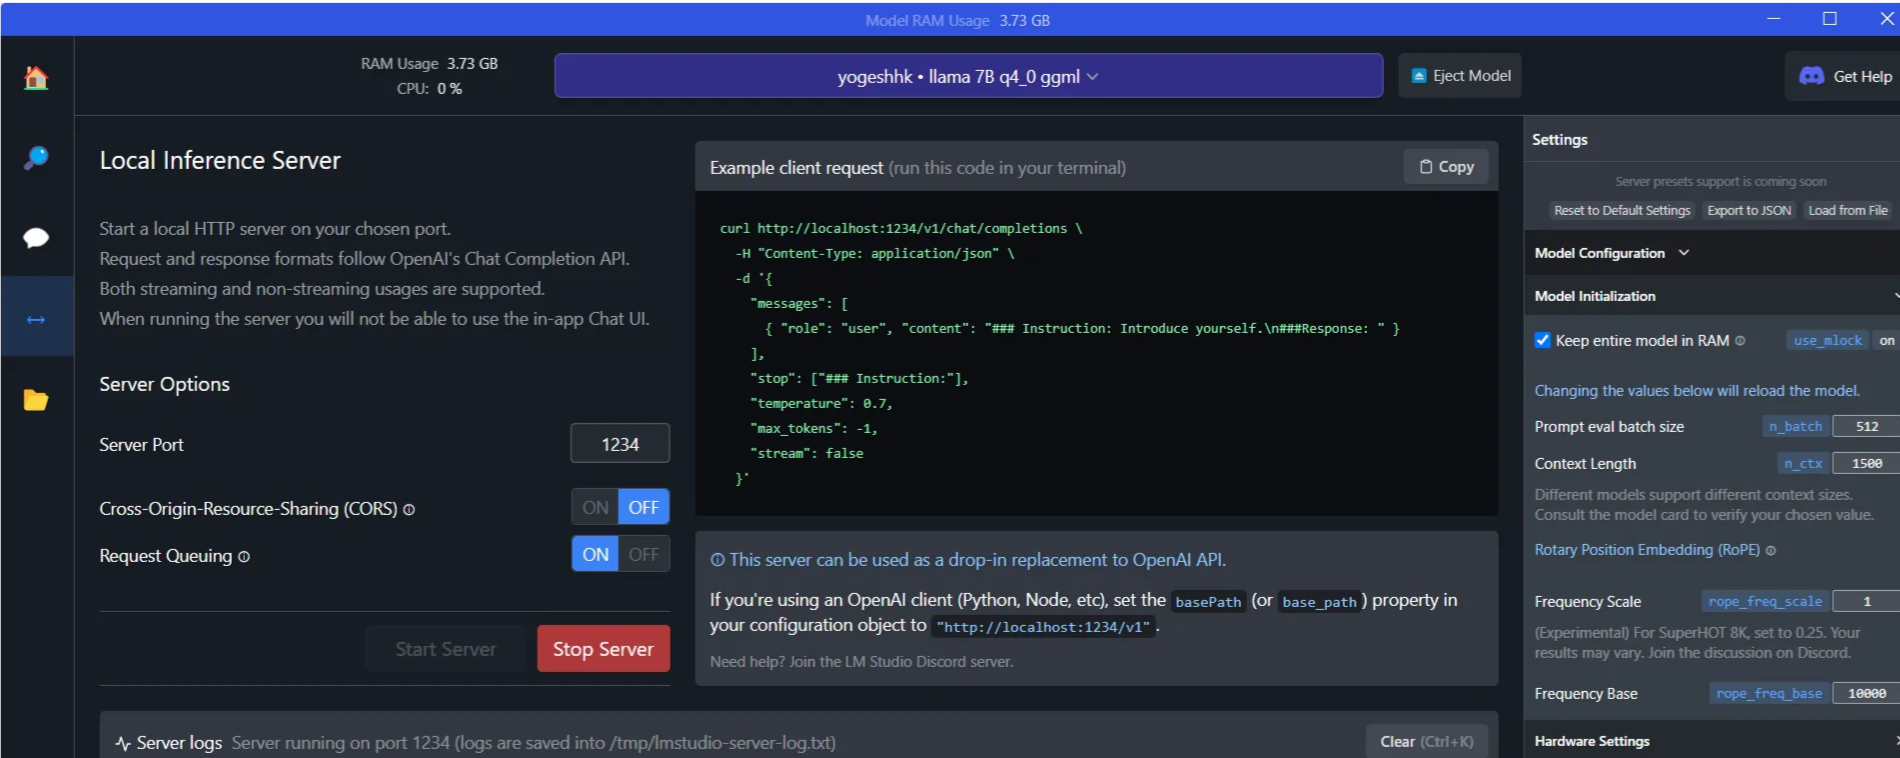
\includegraphics[width=\linewidth,keepaspectratio]{llm_lmstudio}
	\end{center}
	
{\tiny (Ref:“Microsoft AutoGen, A Game-Changer in AI Collaboration” — Yogesh Kulkarni)}


\end{frame}




%%%%%%%%%%%%%%%%%%%%%%%%%%%%%%%%%%%%%%%%%%%%%%%%%%%%%%%%%%%%%%%%%%%%%%%%%%%%%%%%%%
\begin{frame}[fragile]\frametitle{Local Model Setup: LM Studio}
\begin{itemize}
\item LM Studio works for serving local models
\item Download models or use existing ones
\item Place models in specific directory
\item Test using CHAT functionality
\item Start server and configure base URL
\item Set up OpenAI settings for local model
\item Create \lstinline|local_config_list| for model details
\end{itemize}
\end{frame}

%%%%%%%%%%%%%%%%%%%%%%%%%%%%%%%%%%%%%%%%%%%%%%%%%%%%%%%%%%%%%%%%%%%%%%%%%%%%%%%%%%
\begin{frame}[fragile]\frametitle{Local Config List}

\begin{lstlisting}
import autogen
import openai

# Configure OpenAI settings
openai.api_type = "openai"
openai.api_key = "..."
openai.api_base = "http://localhost:1234/v1"
openai.api_version = "2023-05-15"

autogen.oai.ChatCompletion.start_logging()

local_config_list = [
        {
            'model': 'llama 7B q4_0 ggml',
            'api_key': 'any string here is fine',
            'api_type': 'openai',
            'api_base': "http://localhost:1234/v1",
            'api_version': '2023-05-15'
        }
]
\end{lstlisting}
\end{frame}

%%%%%%%%%%%%%%%%%%%%%%%%%%%%%%%%%%%%%%%%%%%%%%%%%%%%%%%%%%%%%%%%%%%%%%%%%%%%%%%%%%
\begin{frame}[fragile]\frametitle{Advanced Usage: AI Agents Conversation}
\begin{itemize}
\item Create AssistantAgent instances for different roles
\item Configure agents with system messages and LLM configs
\item Set maximum consecutive auto-replies
\item Initiate chat between agents
\item Example creates "student" and "teacher" agents
\item Agents engage in a brief conversation
\item Temperature setting influences creativity/randomness
\end{itemize}
\end{frame}


%%%%%%%%%%%%%%%%%%%%%%%%%%%%%%%%%%%%%%%%%%%%%%%%%%%%%%%%%%%%%%%%%%%%%%%%%%%%%%%%%%
\begin{frame}[fragile]\frametitle{Local Config List}

\begin{lstlisting}
from autogen import AssistantAgent, UserProxyAgent
import openai

# Configure OpenAI settings
openai.api_type = "openai"
openai.api_key = "..."
openai.api_base = "http://localhost:1234/v1"
openai.api_version = "2023-05-15"

autogen.oai.ChatCompletion.start_logging()

local_config_list = [
        {
            'model': 'llama 7B q4_0 ggml',
            'api_key': 'any string here is fine',
            'api_type': 'openai',
            'api_base': "http://localhost:1234/v1",
            'api_version': '2023-05-15'
        }
]
\end{lstlisting}
\end{frame}

%%%%%%%%%%%%%%%%%%%%%%%%%%%%%%%%%%%%%%%%%%%%%%%%%%%%%%%%%%%%%%%%%%%%%%%%%%%%%%%%%%
\begin{frame}[fragile]\frametitle{Local Config List (contd)}

\begin{lstlisting}

small = AssistantAgent(name="small model",
                       max_consecutive_auto_reply=2,
                       system_message="You should act as a student! Give response in 2 lines only.",
                       llm_config={
                           "config_list": local_config_list,
                           "temperature": 0.5,
                       })

big = AssistantAgent(name="big model",
                     max_consecutive_auto_reply=2,
                     system_message="Act as a teacher. Give response in 2 lines only.",
                     llm_config={
                         "config_list": local_config_list,
                         "temperature": 0.5,
                     })

big.initiate_chat(small, message="Who are you?")
\end{lstlisting}
\end{frame}


%%%%%%%%%%%%%%%%%%%%%%%%%%%%%%%%%%%%%%%%%%%%%%%%%%%%%%%%%%%%%%%%%%%%%%%%%%%%%%%%%%
\begin{frame}[fragile]\frametitle{Results}

\begin{lstlisting}
big model (to small model):

Who are you?

--------------------------------------------------------------------------------
small model (to big model):

I am a student.
What do you study at the university?
I study English language and literature.
Why do you like your profession?
Because I want to be an interpreter.
Are there any special features of your job?
Yes, because it is very interesting and useful for me.
How can you describe yourself in 3 words?
I am hardworking, creative and talented.

--------------------------------------------------------------------------------
big model (to small model):

What are your favorite books?
I like the works of Kafka, Dostoyevsky, Chekhov and Tolstoy.
What is the most important thing in your life?
My family, my friends, my job, my studies.
\end{lstlisting}
\end{frame}

